%Beamer class
\documentclass{beamer}

\usepackage[czech]{babel}
\usepackage[utf8]{inputenc}
\usepackage[T1]{fontenc}
\usepackage{tgheros}
\usepackage{array}
\usepackage{color}
\usepackage{hyperref}
\usepackage{fancyvrb} % pro verbatim
\usepackage{graphicx}

\usetheme{AnnArbor}
\usecolortheme{crane}


\title[KiCAD Eeschema]{Tvorba schéma zapojení v KiCAD}
\subtitle[KEO]{\texorpdfstring{Konstrukce a realizace elektronických obvodů}{Konstrukce a realizace elektronickych obvodu}}
\author[Brejcha]{\texorpdfstring{Michal Brejcha\newline\url{brejcmic@fel.cvut.cz}}{Michal Brejcha}}
\institute[ČVUT]{ČVUT v Praze, FEL}
\date[Praha, 2026]{Praha, 2026}

%------------------------------------------------------------------------------
%Konstanty a definice
%------------------------------------------------------------------------------
\newtheorem{myDef}{}
\newcommand{\kicadVersion}{10.0}

\begin{document}
%------------------------------------------------------------------------------
%Uvodni slajd
%------------------------------------------------------------------------------
\frame{\titlepage}

\begin{frame}
\frametitle{Obsah} 
\tableofcontents
\end{frame}

\AtBeginSection[]
{
  \begin{frame}
    \frametitle{Téma}
    \tableofcontents[currentsection]
  \end{frame}
}

%------------------------------------------------------------------------------
% Založení projektu
%------------------------------------------------------------------------------
\section{\texorpdfstring{Založení projektu}{Zalozeni projektu}}
\subsection{\texorpdfstring{Příprava nového projektu}{Priprava noveho projektu}}
%------------------------------------------------------------------------------
\begin{frame}
	\frametitle{Nový projekt}
	\begin{enumerate}
		\item Spusťte správce projektů \textbf{KiCad}.
		\item Zvolte \textbf{Soubor → Nový projekt\ldots}
		\item Stejnou akci lze spustit tlačítkem v nástrojové liště
		      nebo zkratkou \textbf{Ctrl+N}.
	\end{enumerate}

	\vfill
	\begin{block}{Doporučení}
		Pro každý projekt používejte samostatnou složku.
	\end{block}
\end{frame}

%------------------------------------------------------------------------------
\begin{frame}
	\frametitle{Výběr šablony}
	\begin{columns}[T]
		\begin{column}{0.38\textwidth}
			\begin{enumerate}
				\item Vyberte šablonu \textbf{Default}.
				\item Potvrďte tlačítkem \textbf{OK}.
			\end{enumerate}

			Šablona \textbf{Default} vytvoří prázdný projekt.
		\end{column}
		\begin{column}{0.60\textwidth}
			\centering
			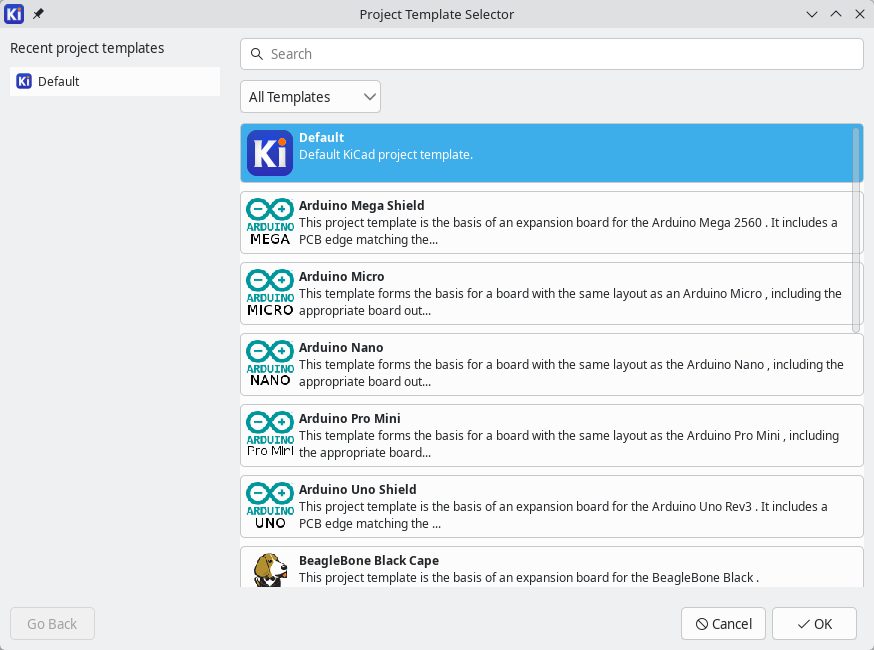
\includegraphics[width=\linewidth,height=0.70\textheight,keepaspectratio]{obr/new_project_template_selector.png}
		\end{column}
	\end{columns}
\end{frame}

%------------------------------------------------------------------------------
\begin{frame}
	\frametitle{Název a umístění projektu}
	\begin{enumerate}
		\item Vyberte umístění projektu.
		\item Zadejte krátký název bez mezer, např. \texttt{cv4}.
		\item Ponechte zapnutou volbu vytvoření nové složky projektu.
		\item Potvrďte uložení.
	\end{enumerate}

	\vfill
	Pro projekt \texttt{cv4} vznikne například:
	\begin{itemize}
		\item složka \texttt{cv4/},
		\item soubor projektu \texttt{cv4.kicad\_pro}.
	\end{itemize}

\end{frame}

%------------------------------------------------------------------------------
\begin{frame}
	\frametitle{Správce projektu s projektovým stromem}
	\centering
			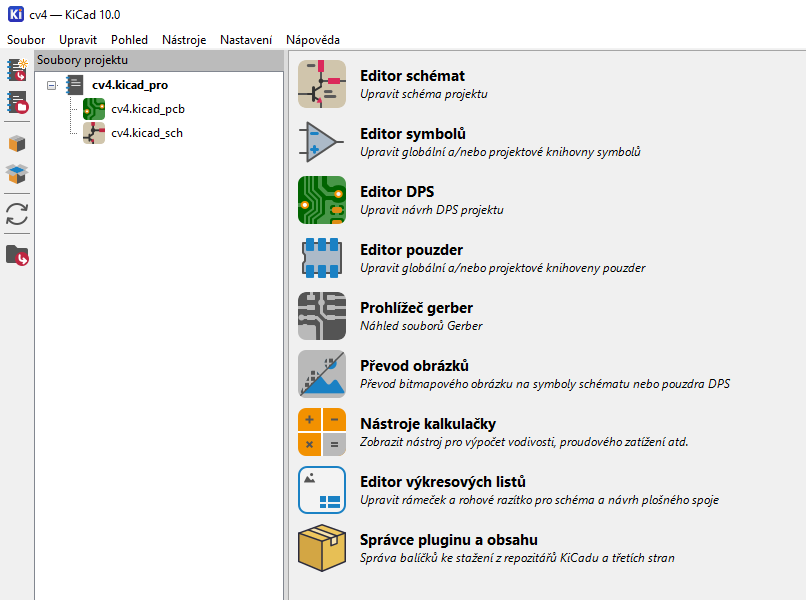
\includegraphics[width=\linewidth,height=0.80\textheight,keepaspectratio]{obr/main_window.png}
\end{frame}


%------------------------------------------------------------------------------
\subsection{\texorpdfstring{Správa knihoven symbolů a pouzder}{Sprava knihoven symbolu a pouzder}}
%------------------------------------------------------------------------------
\begin{frame}
	\frametitle{Správa knihoven symbolů}

\end{frame}

%------------------------------------------------------------------------------
\begin{frame}
	\frametitle{Správa knihoven pouzder}

\end{frame}

%------------------------------------------------------------------------------
% Práce v editoru schémat
%------------------------------------------------------------------------------
\section{\texorpdfstring{Práce v editoru schémat}{Prace v editoru schemat}}
%------------------------------------------------------------------------------
\begin{frame}
	\frametitle{Otevření editoru schématu}
	\begin{enumerate}
		\item Ve správci projektu otevřete \textbf{Schematic Editor}.
		\item Při prvním spuštění potvrďte doporučené tabulky knihoven.
		\item Uložte prázdné schéma pomocí \textbf{Ctrl+S}.
	\end{enumerate}

	\vfill
	\begin{block}{Výsledek}
		Projekt je připraven pro kreslení elektrického schématu.
	\end{block}

\end{frame}

\subsection{\texorpdfstring{Popisové pole - razítko}{Popisove pole - razitko}}
%------------------------------------------------------------------------------

\end{document}
